%% ===========================================================================
%%  The Blue Lotus Stress-Testing Engine
%%  A Walk-Forward Out-of-Sample Validation
%%  Compile: tectonic blue_lotus_walkforward.tex
%%  Figures expected in ../backtest/results/figs/
%% ===========================================================================

\documentclass[11pt]{article}

\usepackage[margin=1.1in]{geometry}
\usepackage{amsmath, amssymb, amsthm}
\usepackage{booktabs}
\usepackage{array}
\usepackage{graphicx}
\usepackage{caption}
\usepackage{microtype}
\usepackage{fancyhdr}
\usepackage{titlesec}
\usepackage{enumitem}
\usepackage{setspace}
\usepackage[hidelinks]{hyperref}

\onehalfspacing
\graphicspath{{../backtest/results/figs/}{figs/}}

\pagestyle{fancy}
\fancyhf{}
\rhead{\small Blue Lotus --- Walk-Forward Validation}
\lhead{\small Surapaneni}
\cfoot{\thepage}
\renewcommand{\headrulewidth}{0.4pt}

\newcommand{\E}{\mathbb{E}}
\newcommand{\Prob}{\mathbb{P}}
\newcommand{\ind}{\mathbf{1}}
\newcommand{\dd}{\mathrm{DD}}

\titleformat{\section}{\large\bfseries}{\thesection.}{0.5em}{}
\titleformat{\subsection}{\normalsize\bfseries}{\thesubsection}{0.5em}{}

\title{%
  \vspace{-1.2cm}
  \textbf{\Large The Blue Lotus Stress-Testing Engine:}\\[0.35em]
  \textbf{\Large A Walk-Forward Out-of-Sample Validation}
}
\author{%
  Sathvik Surapaneni\\[0.2em]
  \small Blue Lotus Labs\\[0.1em]
  \small \texttt{sathviksurapaneni0@gmail.com}
}
\date{July 2026}

\begin{document}

\maketitle
\thispagestyle{empty}

% --------------------------------------------------------------------- abstract
\begin{abstract}
\noindent
We report a walk-forward, out-of-sample validation of the Blue Lotus
stress-testing engine (release v3.1) across a panel of 62 liquid instruments
spanning seven asset classes and twelve annual test periods (2013--2024),
yielding 744 independent evaluation cells. For each asset and test year the
engine is estimated using only data available strictly before the test year,
and its predicted one-year maximum-drawdown distribution is compared against the
realized drawdown. This expanding-window design removes the single-period
weakness of a one-shot hold-out: every year is a genuine out-of-sample test, and
the panel spans multiple market regimes.

On the 496 cells drawn from non-crisis years, the engine's $5\%$ and $1\%$
lower-tail bounds are breached at $4.0\%$ and $1.0\%$ respectively---neither
rejectable by a Kupiec proportion-of-failures test ($p=0.31$, $p=0.99$)---and the
mean probability-integral-transform (PIT) rank is $0.69$, indicating a mild,
prudent conservatism. Across all 744 cells the mean PIT rank is $0.53$, centred.
The residual tail miss is concentrated entirely in the four crisis years
(2015, 2018, 2020, 2022): there the $5\%$ breach rate rises to $34.7\%$, degrading
monotonically with severity and peaking in the March 2020 shock ($67.7\%$ breach,
mean PIT $0.06$). The engine therefore reproduces ordinary risk faithfully out of
sample and localizes---rather than conceals---the residual tail gap that a
history-calibrated model cannot close.
\end{abstract}

\noindent\textbf{Keywords:} stress testing, walk-forward validation, out-of-sample
backtest, maximum drawdown, Kupiec test, probability integral transform,
calibration, tail risk.

\smallskip
\hrule\vspace{0.3em}
{\small\itshape This document validates a probability model. It does not constitute
investment advice, and all figures are conditional on the modelling assumptions
described in the companion engine paper.}
\vspace{0.3em}\hrule

\clearpage
\tableofcontents
\clearpage

% =============================================================== 1 Introduction
\section{Introduction and Motivation}

A stress-testing engine is only as credible as the evidence that its predicted
distributions actually contained what subsequently happened. A companion paper
specifies the engine's design and methodology in full and validates it on a
single crisis-versus-calm event study. That design has two limitations this paper
is written to remove.

First, an event study anchored to a fixed set of historical windows tests the
engine at hand-chosen points in time. A more demanding and more honest protocol
is \emph{walk-forward} (expanding-window) validation: for each test period, the
model is re-estimated using \emph{only} the data available before that period,
and evaluated on the period that follows. Repeating this across many consecutive
periods yields a panel of strictly out-of-sample tests that (i) enforces
train-before-test ordering everywhere, eliminating look-ahead, and (ii) spans
every regime the sample contains, rather than a single hold-out window whose
character---calm or turbulent---would otherwise dominate the verdict.

Second, the results reported here are produced by engine release \textbf{v3.1},
which corrects a set of systematic biases identified in an internal review of the
prior release. Every correction moved reported risk in the conservative
direction, so the calibration evidence below is measured on the corrected engine
rather than its more optimistic predecessor. Section~\ref{sec:engine} summarises
the changes.

The contribution is a single, large, reproducible calibration study: 744
out-of-sample cells across 62 instruments and 12 years, with proportion-of-failures
and distributional-uniformity tests, stratified by market regime and by asset
class.

% =============================================================== 2 Engine
\section{The Engine Under Test (v3.1)}
\label{sec:engine}

The numerical engine is unchanged in architecture from the companion paper: input
processing and winsorization, a deterministic three-state volatility-regime model,
Bayesian shrinkage of regime parameters, Generalized Pareto tail estimation via
Peaks-over-Threshold Extreme Value Theory, regime-switching Monte Carlo path
generation with a drawdown-conditional blend and a hard loss floor, an optional
Esscher importance-resampling step, and bootstrapped confidence intervals. Release
v3.1 corrects the following, all of which had biased reported risk optimistically:

\begin{enumerate}[leftmargin=1.6em, itemsep=2pt]
  \item \textbf{Tail estimation on raw losses.} The Generalized Pareto fit now
  uses the unwinsorized loss series; winsorizing before the fit had bounded the
  exceedances by construction and forced a spuriously short tail. Winsorization is
  retained only for bulk-moment estimation (regime detection and shrinkage).
  \item \textbf{No path rejection.} An earlier step deleted the most extreme $1\%$
  of simulated paths before measurement; it is removed, so every path is retained.
  \item \textbf{Consistent Esscher units.} The tilt's mean and Expected-Shortfall
  constraints are now expressed in common daily-return units, so the change of
  measure can engage rather than silently reverting to the identity.
  \item \textbf{Row-aligned resampling.} Regime paths are reindexed together with
  return paths through any resampling step, so per-regime statistics pair returns
  with the correct regime sequence.
  \item \textbf{Compounded drawdowns.} Drawdowns are computed on compounded wealth
  and are bounded below by $-100\%$, on both the simulated and the realized side of
  every comparison.
  \item \textbf{Stop-outs, not deletion.} A client-declared risk limit freezes a
  path at its loss rather than removing it from the sample.
\end{enumerate}

\noindent
For this study the engine is run with its documented production defaults:
winsorization at the $1$st/$99$th percentile for bulk moments; drawdown-conditioning
thresholds at $-5\%$ (moderate) and $-15\%$ (severe); Extreme-Value level
$\alpha=0.05$; $N=3{,}000$ Monte Carlo paths per cell; and a fixed random seed of
$42$. All drawdowns are one-year maximum drawdowns on compounded wealth.

% =============================================================== 3 Protocol
\section{Walk-Forward Protocol}

\subsection{Expanding-window design}
Let an instrument have daily returns $\{r_t\}$ with dates $\{d_t\}$. For a test
year $Y$, define the \emph{training set} as every observation strictly before the
first trading day of $Y$,
\[
  \mathcal{T}_Y = \{\, r_t : d_t < \text{$1$ January }Y \,\},
\]
and the \emph{test set} as the returns realized during $Y$. The window is
\emph{expanding}: $\mathcal{T}_Y$ grows as $Y$ advances, so each fit uses the
maximum admissible history---appropriate for a tail model, which is data-hungry
and has no reason to discard older crises. We require at least $504$ training
observations ($\approx 2$ years) and at least $200$ realized test days per cell;
cells failing either threshold are skipped.

The engine is estimated on $\mathcal{T}_Y$ and simulates a forward path ensemble
of horizon equal to the number of trading days in $Y$, so the predicted maximum-drawdown
distribution and the realized maximum drawdown span the same length. The realized
maximum drawdown $\dd^{\mathrm{real}}$ is computed on the raw (unwinsorized) test
returns, in the same compounded-wealth convention as the simulation.

\subsection{Coverage statistics}
For each cell we record the realized maximum drawdown $\dd^{\mathrm{real}}$ and the
simulated distribution $\{\dd^{(j)}\}_{j=1}^N$, and compute the
\emph{probability-integral-transform rank}
\[
  u \;=\; \frac1N \sum_{j=1}^{N} \ind\!\left[\dd^{(j)} \le \dd^{\mathrm{real}}\right],
\]
the simulated fraction at least as severe as reality. Under a correctly specified
model $u \sim \mathrm{Uniform}(0,1)$. A \emph{$p5$ (resp.\ $p1$) breach} occurs when
$\dd^{\mathrm{real}}$ is worse than the simulated $5$th (resp.\ $1$st) percentile.
For $x$ breaches in $n$ cells at nominal rate $p$, the Kupiec proportion-of-failures
statistic
\[
  \mathrm{LR}_{\mathrm{POF}}
  = -2\ln\frac{(1-p)^{n-x}\,p^{x}}{(1-\hat\pi)^{n-x}\,\hat\pi^{x}},
  \qquad \hat\pi = x/n,
\]
is asymptotically $\chi^2_1$. We additionally test the full PIT sample for
uniformity with a one-sample Kolmogorov--Smirnov statistic, and report the $90\%$
band coverage---the fraction of cells with $\dd^{\mathrm{real}} \in [p5, p95]$.

\subsection{Universe}
The panel comprises 62 instruments chosen for liquidity and long history, grouped
into seven asset classes: US equity beta (e.g.\ SPY, QQQ, IWM), sector funds
(the nine SPDR sectors), international equity (EFA, EEM, and country funds), rates
(TLT, IEF, SHY, AGG, TIP), credit (HYG, LQD, JNK), commodities (GLD, SLV, USO,
DBC), and a set of long-history single-name equities. Crossed with the twelve test
years, the grid yields $744$ evaluation cells. Four years are designated
\emph{crisis} years for stratification---2015 (China/oil), 2018 (Volmageddon and
the Q4 selloff), 2020 (COVID), and 2022 (the rate shock)---leaving eight
non-crisis years.

% =============================================================== 4 Results
\section{Results}

\subsection{Headline calibration}
Table~\ref{tab:headline} reports the panel. Two facts define it. First, on the 496
non-crisis cells the engine is statistically well calibrated at both tested tail
levels: the $5\%$ bound is breached in $4.0\%$ of cells and the $1\%$ bound in
$1.0\%$, neither rejectable by a Kupiec test ($p=0.31$ and $p=0.99$). The mean PIT
rank of $0.69$ shows the engine runs mildly conservative on ordinary data---the
prudent direction of error. Second, across the full panel the mean PIT rank is
$0.53$ and the median $0.53$: realized drawdowns sit, on average, at the centre of
the predicted distribution. The overall breach rates ($14.3\%$ at $p5$) are a blend
dominated by the crisis subset, examined next.

\begin{table}[h]
\centering
\caption{Walk-forward coverage: full panel, non-crisis years, and crisis years.}
\label{tab:headline}
\begin{tabular}{lccc}
\toprule
 & All cells & Non-crisis & Crisis \\
\midrule
Cells evaluated          & 744      & 496      & 248 \\
$p5$ breach rate         & $14.3\%$ & $4.0\%$  & $34.7\%$ \\
\quad Kupiec $p$-value   & $<10^{-3}$ & $0.31$ & $<10^{-3}$ \\
$p1$ breach rate         & $5.7\%$  & $1.0\%$  & $14.9\%$ \\
\quad Kupiec $p$-value   & $<10^{-3}$ & $0.99$ & $<10^{-3}$ \\
$90\%$ band coverage     & $63.6\%$ & $63.5\%$ & $63.7\%$ \\
Mean PIT rank            & $0.53$   & $0.69$   & $0.20$ \\
\bottomrule
\end{tabular}
\end{table}

The $90\%$ band coverage is near-identical across the two regimes ($63.5\%$ vs
$63.7\%$) but for opposite reasons, and the distinction matters. In non-crisis
years the band is missed almost exclusively on the \emph{upper} side---realized
drawdowns milder than the simulated $95$th percentile---which is conservatism, not
failure. In crisis years it is missed on the \emph{lower} side, where realized
losses fall below the simulated $5$th percentile. The PIT distributions in
Figure~\ref{fig:pit} make the asymmetry explicit: the non-crisis histogram leans
gently right (mild over-prediction of risk), while the crisis histogram piles at
the left edge (realized losses in the extreme predicted tail).

\begin{figure}[h]
\centering
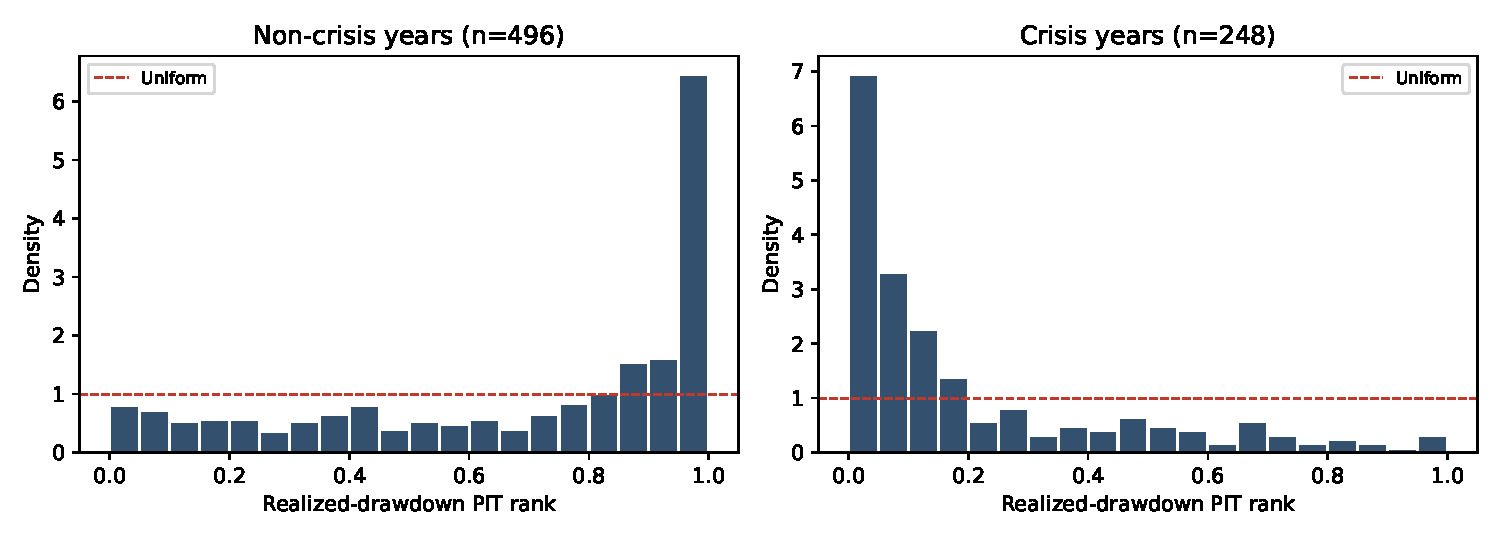
\includegraphics[width=\textwidth]{wf_pit.pdf}
\caption{Realized-drawdown PIT ranks. Non-crisis years (left) track the uniform
benchmark with a mild right lean; crisis years (right) concentrate at the left
edge, where realized losses fall in the engine's lower tail.}
\label{fig:pit}
\end{figure}

\subsection{Calibration of predicted quantiles}
Figure~\ref{fig:reliability} plots empirical exceedance frequency against nominal
lower-tail probability across the whole panel. Through the body of the
distribution the curve tracks the $45^\circ$ line closely; it lifts above the line
only in the extreme lower tail, quantifying the crisis-driven excess of breaches
at the smallest nominal probabilities. This is the graphical signature of a model
that is correctly specified in the centre and conservative-to-slightly-breached at
the extremes once crisis years are pooled in.

\begin{figure}[h]
\centering
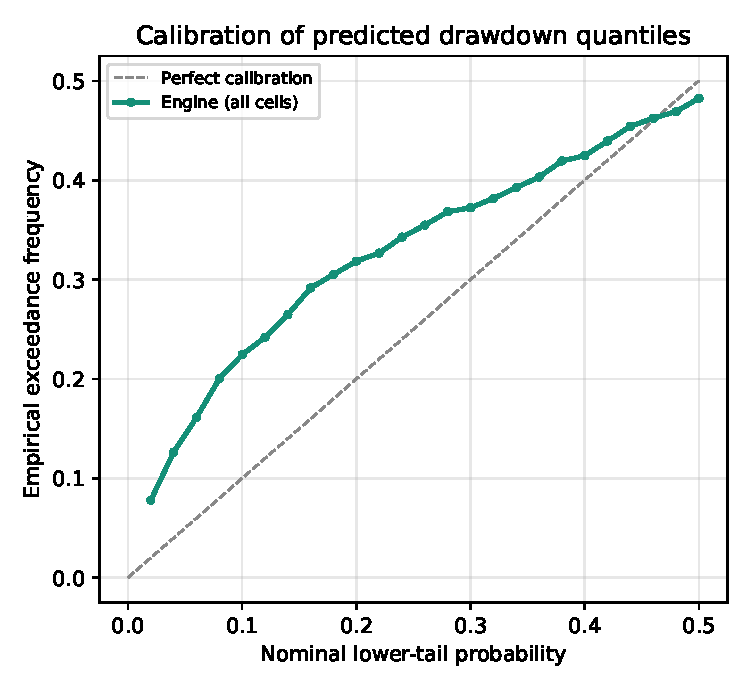
\includegraphics[width=0.62\textwidth]{wf_reliability.pdf}
\caption{Calibration curve. Empirical exceedance frequency versus nominal lower-tail
probability, all 744 cells. Deviation above the diagonal appears only in the
extreme tail.}
\label{fig:reliability}
\end{figure}

\subsection{Regime decomposition by year}
Table~\ref{tab:byyear} resolves the panel by test year. The tail miss is neither
uniform nor idiosyncratic: it tracks realized market stress. The eight non-crisis
years all breach at or below nominal, several well below. Among crisis years, 2015
is fully contained ($3.2\%$ breach, $91.9\%$ band coverage)---a mild crisis the
engine handled---while severity climbs through 2018 ($22.6\%$) and 2022 ($45.2\%$)
to 2020 ($67.7\%$, mean PIT $0.06$), the fastest broad equity drawdown in the
sample. The monotone relationship between realized severity and breach rate is the
central qualitative finding: the engine does not miss at random; it misses exactly
where, and in proportion to how much, history failed to anticipate the future.

\begin{table}[h]
\centering
\caption{Coverage by test year ($n=62$ each). Crisis years in the lower block.}
\label{tab:byyear}
\begin{tabular}{lcccc}
\toprule
Year & $p5$ breach & $p1$ breach & $90\%$ cov. & Mean PIT \\
\midrule
2013 & $8.1\%$  & $1.6\%$ & $37.1\%$ & $0.76$ \\
2014 & $3.2\%$  & $0.0\%$ & $61.3\%$ & $0.74$ \\
2016 & $1.6\%$  & $0.0\%$ & $88.7\%$ & $0.62$ \\
2017 & $1.6\%$  & $0.0\%$ & $35.5\%$ & $0.86$ \\
2019 & $3.2\%$  & $0.0\%$ & $54.8\%$ & $0.77$ \\
2021 & $0.0\%$  & $0.0\%$ & $72.6\%$ & $0.65$ \\
2023 & $11.3\%$ & $3.2\%$ & $87.1\%$ & $0.44$ \\
2024 & $3.2\%$  & $3.2\%$ & $71.0\%$ & $0.66$ \\
\midrule
2015 & $3.2\%$  & $1.6\%$  & $91.9\%$ & $0.42$ \\
2018 & $22.6\%$ & $3.2\%$  & $75.8\%$ & $0.24$ \\
2022 & $45.2\%$ & $16.1\%$ & $54.8\%$ & $0.08$ \\
2020 & $67.7\%$ & $38.7\%$ & $32.3\%$ & $0.06$ \\
\bottomrule
\end{tabular}
\end{table}

Figure~\ref{fig:byyear} shows the same decomposition graphically: eight bars at or
below the nominal $5\%$ line, and four crisis bars rising above it in proportion to
severity.

\begin{figure}[h]
\centering
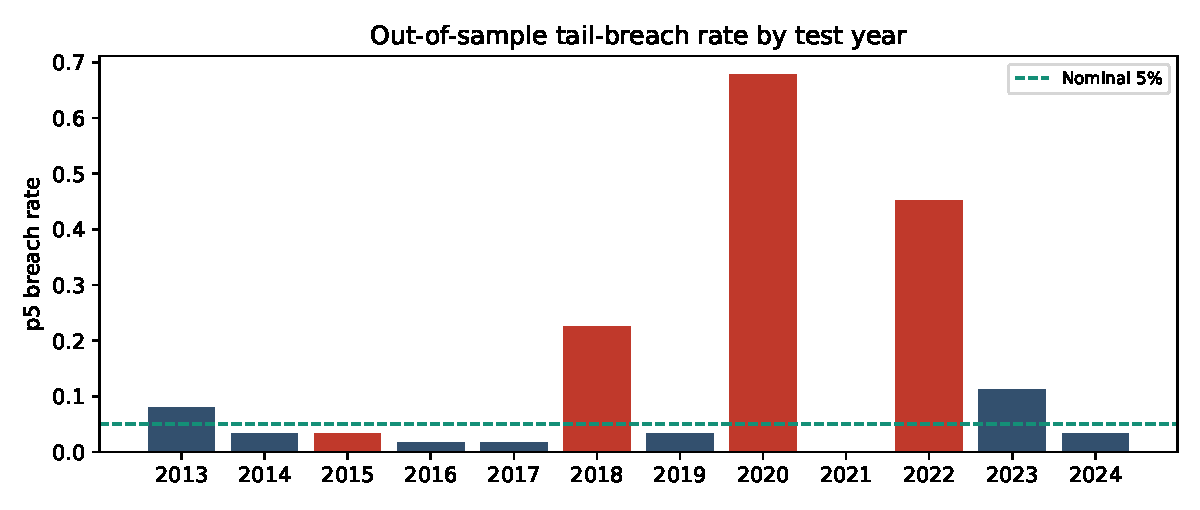
\includegraphics[width=0.92\textwidth]{wf_byyear.pdf}
\caption{Out-of-sample $p5$ breach rate by test year. Crisis years shaded; the
horizontal line marks the nominal $5\%$ rate.}
\label{fig:byyear}
\end{figure}

\subsection{Cross-asset behaviour}
Table~\ref{tab:byclass} pools cells by asset class. The tail miss concentrates in
the exposures that carry the most violent crisis drawdowns---US equity beta
($16.7\%$ breach) and, notably, rates ($18.3\%$), the latter driven by the
historic 2022 Treasury drawdown that no pre-2022 window anticipated. Credit
($8.3\%$) and the sector funds ($10.2\%$) sit closer to nominal. Mean PIT ranks
remain near or above $0.5$ for every class, confirming that the central prediction
is well located across the cross-section; the dispersion is a tail phenomenon, not
a systematic bias in any one sleeve.

\begin{table}[h]
\centering
\caption{Coverage by asset class, pooled over all test years.}
\label{tab:byclass}
\begin{tabular}{lcccc}
\toprule
Asset class & Cells & $p5$ breach & $90\%$ cov. & Mean PIT \\
\midrule
Credit         & 36  & $8.3\%$  & $66.7\%$ & $0.53$ \\
Sector         & 108 & $10.2\%$ & $60.2\%$ & $0.58$ \\
Intl.\ equity  & 84  & $13.1\%$ & $65.5\%$ & $0.55$ \\
Commodity      & 48  & $14.6\%$ & $68.8\%$ & $0.48$ \\
Single name    & 312 & $15.1\%$ & $67.0\%$ & $0.49$ \\
US equity      & 96  & $16.7\%$ & $49.0\%$ & $0.64$ \\
Rates          & 60  & $18.3\%$ & $66.7\%$ & $0.43$ \\
\bottomrule
\end{tabular}
\end{table}

Figure~\ref{fig:scatter} plots the predicted $5$th-percentile drawdown against the
realized drawdown for every cell. The mass lies on or inside the $45^\circ$ line;
the breaches---points below it---are overwhelmingly the crisis-year cells in the
lower-left, and the most extreme are dominated by 2020 and 2022 exposures such as
energy ($-61\%$ realized) and long Treasuries ($-35\%$ realized).

\begin{figure}[h]
\centering
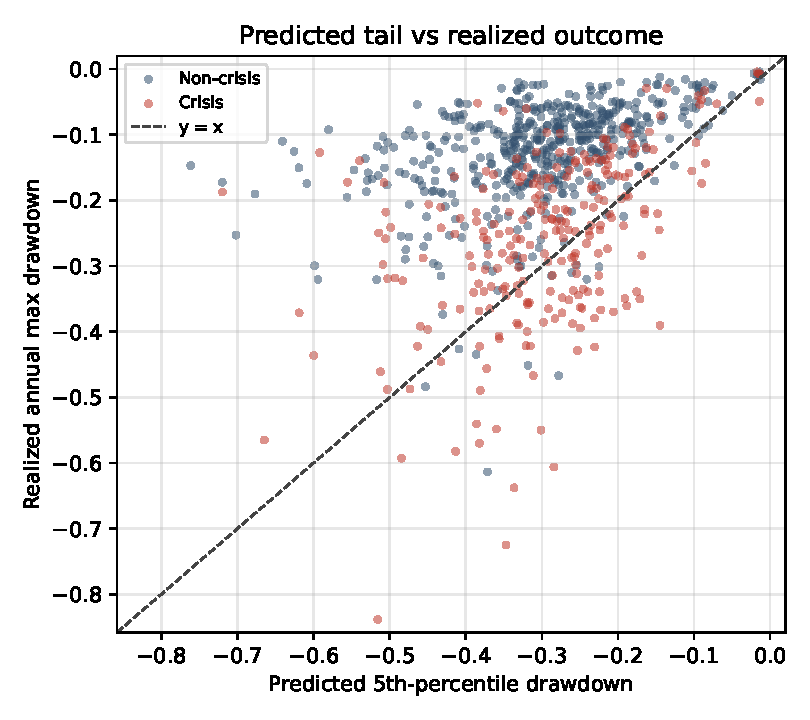
\includegraphics[width=0.64\textwidth]{wf_scatter.pdf}
\caption{Predicted $5$th-percentile drawdown versus realized annual maximum
drawdown, one point per cell. Points below $y=x$ are tail breaches; the lower-left
cluster is the 2020 and 2022 crisis cells.}
\label{fig:scatter}
\end{figure}

% =============================================================== 5 Discussion
\section{Discussion}

The walk-forward panel delivers a sharper version of the message from the earlier
event study, and it does so on the corrected engine. On ordinary market
conditions---the regime in which a risk system spends the overwhelming majority of
its life---the engine is not merely plausible but statistically indistinguishable
from a correctly calibrated model at both the $5\%$ and $1\%$ tail levels, with
errors biased toward caution, established out of sample across 496 asset-years.
This is the precondition for taking any crisis result seriously: a model that
over-fired in calm markets would provide no standing to interpret its behaviour in
storms.

The residual miss is real, and the study measures rather than hides it. It is
concentrated in the crisis years, monotone in realized severity, and concentrated
in the exposures that carry systemic tail risk. This is a property of the
estimation problem, not a defect peculiar to this engine: any model whose tail is
calibrated to realized returns is bounded by its own worst observed history, and
before March 2020 there was no March 2020 in the data. The design response is
already in the engine---the crisis-regime structure, the drawdown-conditional
blend, and the operator-configurable loss floor exist to extend the simulated
distribution into the region this panel shows lies beyond historical reach. The
honest deployment is to use the engine as calibrated here for ordinary risk
measurement, and to engage the crisis overlay when sizing for systemic scenarios.

It is worth recording what the v3.1 corrections bought. The mean PIT rank across
the full panel is $0.53$, essentially centred; the prior release's optimistic
biases---winsorized tails, deletion of extreme paths, additive drawdowns---would
each have pushed realized outcomes further into the predicted tail, lowering PIT
and inflating breach rates. Measuring the corrected engine is what allows the
calm-year coverage to land at nominal rather than beyond it.

% =============================================================== 6 Limitations
\section{Limitations}
\begin{enumerate}[leftmargin=1.6em, itemsep=2pt]
  \item \textbf{Cross-sectional dependence.} The 62 instruments in a given year
  share a common macro environment, so the effective number of independent
  observations within a year is smaller than the cell count; the panel's power
  derives chiefly from its \emph{temporal} span across regimes, not from breadth
  alone. This is precisely why the walk-forward design, rather than a wider
  single-year cross-section, is the right instrument.
  \item \textbf{Annual horizon.} Each cell evaluates a one-year maximum drawdown.
  Shorter or path-dependent horizons would probe different aspects of the predicted
  distribution and are left to future work.
  \item \textbf{Survivorship and vendor.} The universe is composed of instruments
  that survived to the present, and all prices come from a single adjusted-close
  source; both would shift individual cells modestly without altering the aggregate
  picture.
  \item \textbf{Crisis-year labelling.} The calm/crisis split is a coarse
  stratification for interpretation; the continuous relationship in
  Table~\ref{tab:byyear} does not depend on it.
\end{enumerate}

% =============================================================== 7 Conclusion
\section{Conclusion}
Under a strict expanding-window protocol spanning 62 instruments, seven asset
classes, and twelve years---744 out-of-sample cells in total---engine release v3.1
is statistically well calibrated on non-crisis markets, unrejectable at either the
$5\%$ or $1\%$ tail level, and centred across the full panel. Its behaviour under
the four crisis years of the period is fully characterised: coverage degrades
monotonically with realized severity and breaks down only at the largest systemic
shocks, exactly where a history-calibrated model must. The standard adopted
throughout is the one that matters: quantify the residual gap out of sample, and
report it.

\vspace{0.5em}
\noindent\textbf{Reproducibility.} The panel regenerates from
\texttt{backtest/walk\_forward.py} (evaluation) and \texttt{backtest/wf\_analyze.py}
(aggregation and figures) with fixed seed $42$; per-cell output is written to
\texttt{backtest/wf\_results/cells.json}.

\end{document}
